\documentclass[a4paper,11pt]{article}
\input{/home/tof/Documents/Cozy/latex-include/preambule_lua.tex}
\newcommand{\showprof}{show them}  % comment this line if you don't want to see todo environment
\fancyhead[L]{Exercices graphes représentation - correction}
\newdate{madate}{10}{09}{2020}
%\fancyhead[R]{\displaydate{madate}} %\today
%\fancyhead[R]{Seconde - SNT}
%\fancyhead[R]{Première - NSI}
\fancyhead[R]{Terminale - NSI}
\fancyfoot[L]{~\\Christophe Viroulaud}
\AtEndDocument{\label{lastpage}}
\fancyfoot[C]{\textbf{Page \thepage/\pageref{lastpage}}}
\fancyfoot[R]{\includegraphics[width=2cm,align=t]{/home/tof/Documents/Cozy/latex-include/cc.png}}
\usepackage{tikz}
\begin{document}
\begin{Form}
\begin{exo}
\begin{enumerate}
\item Matrice d'adjacence
$$\begin{pmatrix}
0 & 1 & 1 & 1 & 0 & 0 \\
1 & 0 & 0 & 1 & 0 & 0 \\
1 & 0 & 0 & 0 & 1 & 0 \\
1 & 1 & 0 & 0 & 0 & 0 \\
0 & 0 & 1 & 1 & 0 & 0 \\
0 & 0 & 0 & 0 & 0 & 0 \\
\end{pmatrix}$$
\begin{lstlisting}
g = [[0, 1, 1, 1, 0, 0],
      [1, 0, 0, 1, 0, 0],
      [1, 0, 0, 0, 1, 0],
      [1, 1, 0, 0, 0, 0],
      [0, 0, 1, 1, 0, 0],
      [0, 0, 0, 0, 0, 0]]
\end{lstlisting}
\item Dictionnaire d'adjacence
\begin{lstlisting}
g = {"A": {"B", "C", "D"},
      "B": {"A", "D"},
      "C": {"A", "E"},
      "D": {"A", "B", "E"},
      "E": {"C", "D"},
      "F": set()} # par défaut {} représente un dictionnaire
\end{lstlisting}
\end{enumerate}
\end{exo}
\begin{exo}
\begin{center}
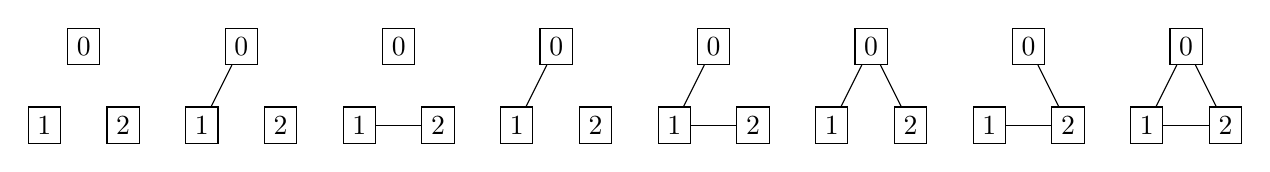
\begin{tikzpicture}
\node[draw] (0) at (-11.5,1) {0};
\node[draw] (1) at (-12,0) {1};
\node[draw] (2) at (-11,0) {2};

\node[draw] (0a) at (-9.5,1) {0};
\node[draw] (1a) at (-10,0) {1};
\node[draw] (2a) at (-9,0) {2};
\draw (0a) -- (1a);

\node[draw] (0b) at (-7.5,1) {0};
\node[draw] (1b) at (-8,0) {1};
\node[draw] (2b) at (-7,0) {2};
\draw (1b) -- (2b);

\node[draw] (0c) at (-5.5,1) {0};
\node[draw] (1c) at (-6,0) {1};
\node[draw] (2c) at (-5,0) {2};
\draw (1c) -- (0c);

\node[draw] (0d) at (-3.5,1) {0};
\node[draw] (1d) at (-4,0) {1};
\node[draw] (2d) at (-3,0) {2};
\draw (1d) -- (0d);
\draw (1d) -- (2d);

\node[draw] (0e) at (-1.5,1) {0};
\node[draw] (1e) at (-2,0) {1};
\node[draw] (2e) at (-1,0) {2};
\draw (1e) -- (0e);
\draw (0e) -- (2e);

\node[draw] (0f) at (0.5,1) {0};
\node[draw] (1f) at (0,0) {1};
\node[draw] (2f) at (1,0) {2};
\draw (1f) -- (2f);
\draw (0f) -- (2f);

\node[draw] (0f) at (2.5,1) {0};
\node[draw] (1f) at (2,0) {1};
\node[draw] (2f) at (3,0) {2};
\draw (1f) -- (0f);
\draw (0f) -- (2f);
\draw (1f) -- (2f);
\end{tikzpicture}
\end{center}
\end{exo}
\begin{exo}
\lstinputlisting[firstline=37,lastline=55]{"scripts/mod_graphe.py"}
\end{exo}
\begin{exo}
\lstinputlisting[firstline=57,lastline=58]{"scripts/mod_graphe.py"}
\end{exo}
\begin{exo}
\lstinputlisting[firstline=60,lastline=61]{"scripts/mod_graphe.py"}
\end{exo}
\begin{exo}
\begin{enumerate}
\item $\sum{degres} = 2×\sum{aretes}$ On remarque également que la somme des degrés est nécessairement paire.
\item Cette propriété nous est utile dans l'écriture de la méthode.
\lstinputlisting[firstline=63,lastline=67]{"scripts/mod_graphe.py"}
\end{enumerate}
\end{exo}
\begin{exo}
\lstinputlisting[firstline=69,lastline=74]{"scripts/mod_graphe.py"}
\end{exo}
\end{Form}
\end{document}